\documentclass[11pt,aspectratio=169]{beamer}

\usetheme{metropolis}
\usepackage[utf8]{inputenc}
\usepackage[T1]{fontenc}
\usepackage[french]{babel}
\usepackage{graphicx}
\usepackage{booktabs}
\usepackage{xcolor}
\usepackage{amsmath}
\usepackage{tikz}

\graphicspath{{figures/}}

% Couleurs personnalisées (ESP/UCAD)
\definecolor{espblue}{RGB}{20,80,160}
\definecolor{espgold}{RGB}{210,160,40}
\definecolor{drop}{RGB}{200,40,40}
\setbeamercolor{frametitle}{bg=espblue,fg=white}
\setbeamercolor{progress bar}{fg=espgold}
\setbeamercolor{title separator}{fg=espgold}

\title{Détection d'objets en temps réel}
\subtitle{Étude comparative \textbf{YOLO11n} vs \textbf{RF-DETR-S}\\Application à la langue des signes américaine (ASL)}
\date{\today}
\author{\textbf{Mouhamed Lamine Faye} \and \textbf{Pape Moussa Mbengue} \and \textbf{Mouhamadou Wally Ndour}}
\institute{DIC3 -- Génie Informatique \\ École Supérieure Polytechnique \\ Université Cheikh Anta Diop de Dakar}

\begin{document}

%% --------------------------------------------------------------------
\maketitle

%% --------------------------------------------------------------------
\begin{frame}{Plan}
  \tableofcontents
\end{frame}

%% ====================================================================
\section{Contexte \& Problématique}

\begin{frame}{Pourquoi la détection d'objets ?}
  \begin{columns}[T,onlytextwidth]
    \column{.55\textwidth}
    \begin{itemize}
      \item La \textbf{détection} localise et classe simultanément (vs classification simple).
      \item Deux familles dominantes :
      \begin{itemize}
        \item CNN one-shot \emph{(YOLO)} : rapidité.
        \item Transformeurs \emph{(DETR / RF-DETR)} : précision \& robustesse.
      \end{itemize}
      \item Mais comment choisir en pratique ?
    \end{itemize}
    \column{.40\textwidth}
    \centering
    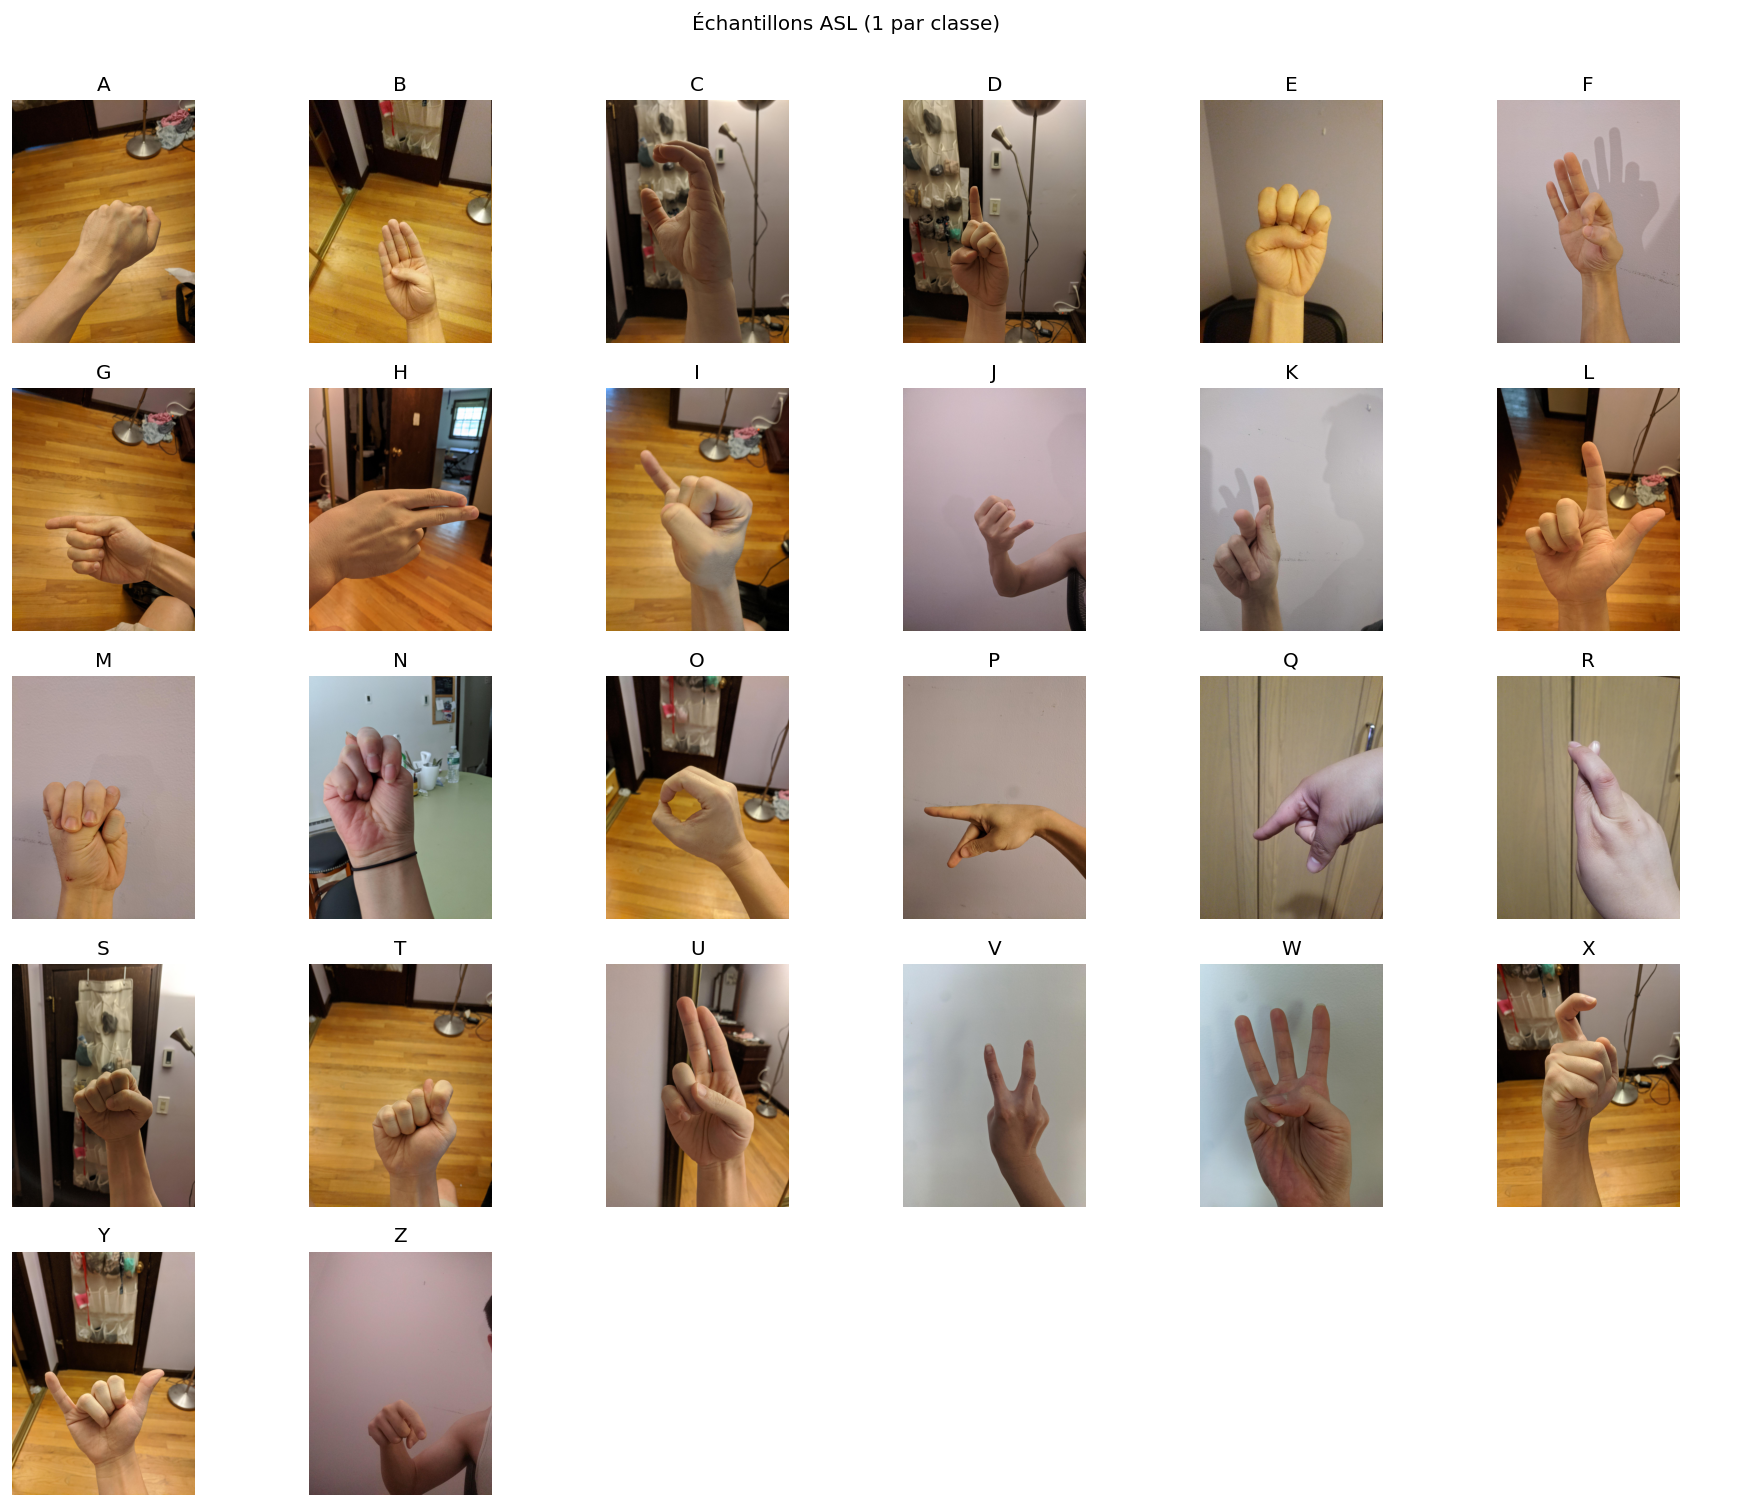
\includegraphics[width=\linewidth]{fig_samples_grid.png}\\
    {\tiny Échantillons du dataset ASL}
  \end{columns}
\end{frame}

\begin{frame}{Cas d'usage : Inclusion}
  \begin{columns}[T,onlytextwidth]
    \column{.55\textwidth}
    \begin{block}{Reconnaissance des 26 lettres ASL}
      \begin{itemize}
        \item Application d'\textbf{accessibilité} pour personnes sourdes/malentendantes.
        \item Démo \textbf{webcam temps réel} : épellation par geste.
      \end{itemize}
    \end{block}

    \begin{alertblock}{Question de recherche}
      Sur un dataset modeste (~1700 images, 26 classes), quel modèle offre le meilleur
      \textbf{compromis} précision / vitesse / \textbf{robustesse} ?
    \end{alertblock}

    \column{.40\textwidth}
    \centering
    \begin{tikzpicture}
      \node[draw=espblue,line width=1.5pt,rounded corners=8pt,inner sep=10pt,fill=espblue!10]
        {\Huge\textbf{A--Z}};
    \end{tikzpicture}\\[6pt]
    {\small 26 lettres signées}
  \end{columns}
\end{frame}

%% ====================================================================
\section{Dataset \& Méthodologie}

\begin{frame}{Dataset — American Sign Language Letters}
  \begin{columns}[T,onlytextwidth]
    \column{.5\textwidth}
    \begin{itemize}
      \item Source : Roboflow Universe (David Lee).
      \item \textbf{1\,720 images} en RGB, 26 classes.
      \item Splits \textbf{train / valid / test} : 504 / 144 / 72.
      \item Format : YOLO + COCO.
      \item Augmentations natives (mosaic, flips, jitter HSV).
    \end{itemize}
    \column{.5\textwidth}
    \centering
    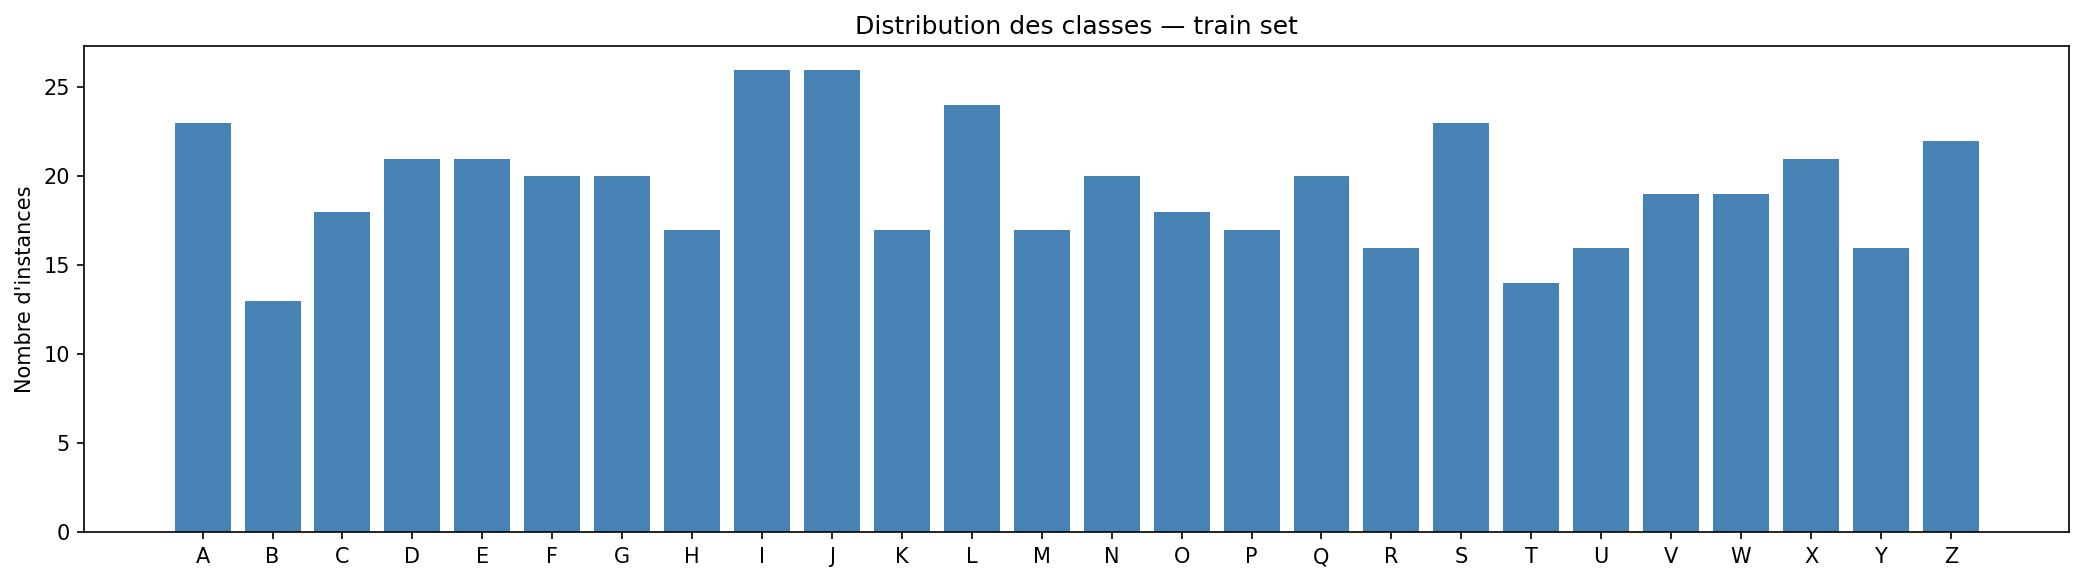
\includegraphics[width=\linewidth]{fig_class_distribution.png}\\
    {\tiny Distribution des classes — train set}
  \end{columns}
\end{frame}

\begin{frame}{Modèles comparés}
  \begin{columns}[T,onlytextwidth]
    \column{.48\textwidth}
    \begin{block}{YOLO11n — Ultralytics (2024)}
      \begin{itemize}
        \item CNN one-shot (CSPDarknet + PANet).
        \item NMS post-traitement.
        \item Variante \emph{nano} : 2.6 M paramètres, $\sim$5 MB.
        \item Pré-entraîné COCO.
      \end{itemize}
    \end{block}

    \column{.48\textwidth}
    \begin{block}{RF-DETR-S — Roboflow (ICLR 2026)}
      \begin{itemize}
        \item Transformeur à backbone \textbf{DINOv2}.
        \item Pas de NMS (\emph{set prediction}).
        \item Variante \emph{small} : $\sim$30 M paramètres, $\sim$122 MB.
        \item SOTA sur COCO ($>$60 mAP).
      \end{itemize}
    \end{block}
  \end{columns}
  \medskip
  \centering\textbf{Comparaison équitable :} mêmes splits, seed 42, $640\times 640$.
\end{frame}

\begin{frame}{Méthodologie}
  \begin{columns}[T,onlytextwidth]
    \column{.48\textwidth}
    \begin{block}{Entraînement (Google Colab T4)}
      \begin{itemize}
        \item YOLO : 50 epochs, batch 32.
        \item RF-DETR : 30 epochs, batch 4 ($\times$4 grad accum).
        \item Optimiseur AdamW, LR cosinus.
      \end{itemize}
    \end{block}

    \column{.48\textwidth}
    \begin{block}{Évaluation}
      \begin{itemize}
        \item Précision : mAP@0.5, mAP@0.5:0.95, P, R, F1.
        \item Complexité : latence, FPS, taille.
        \item \textbf{Robustesse} : 5 dégradations photométriques :
        \begin{itemize}
          \item Luminosité $\gamma\in\{0.5, 0.75, 1.5\}$
          \item Bruit gaussien $\sigma\in\{15, 35\}$
        \end{itemize}
      \end{itemize}
    \end{block}
  \end{columns}
\end{frame}

%% ====================================================================
\section{Résultats}

\begin{frame}{Convergence des modèles}
  \begin{columns}[T,onlytextwidth]
    \column{.48\textwidth}
    \centering
    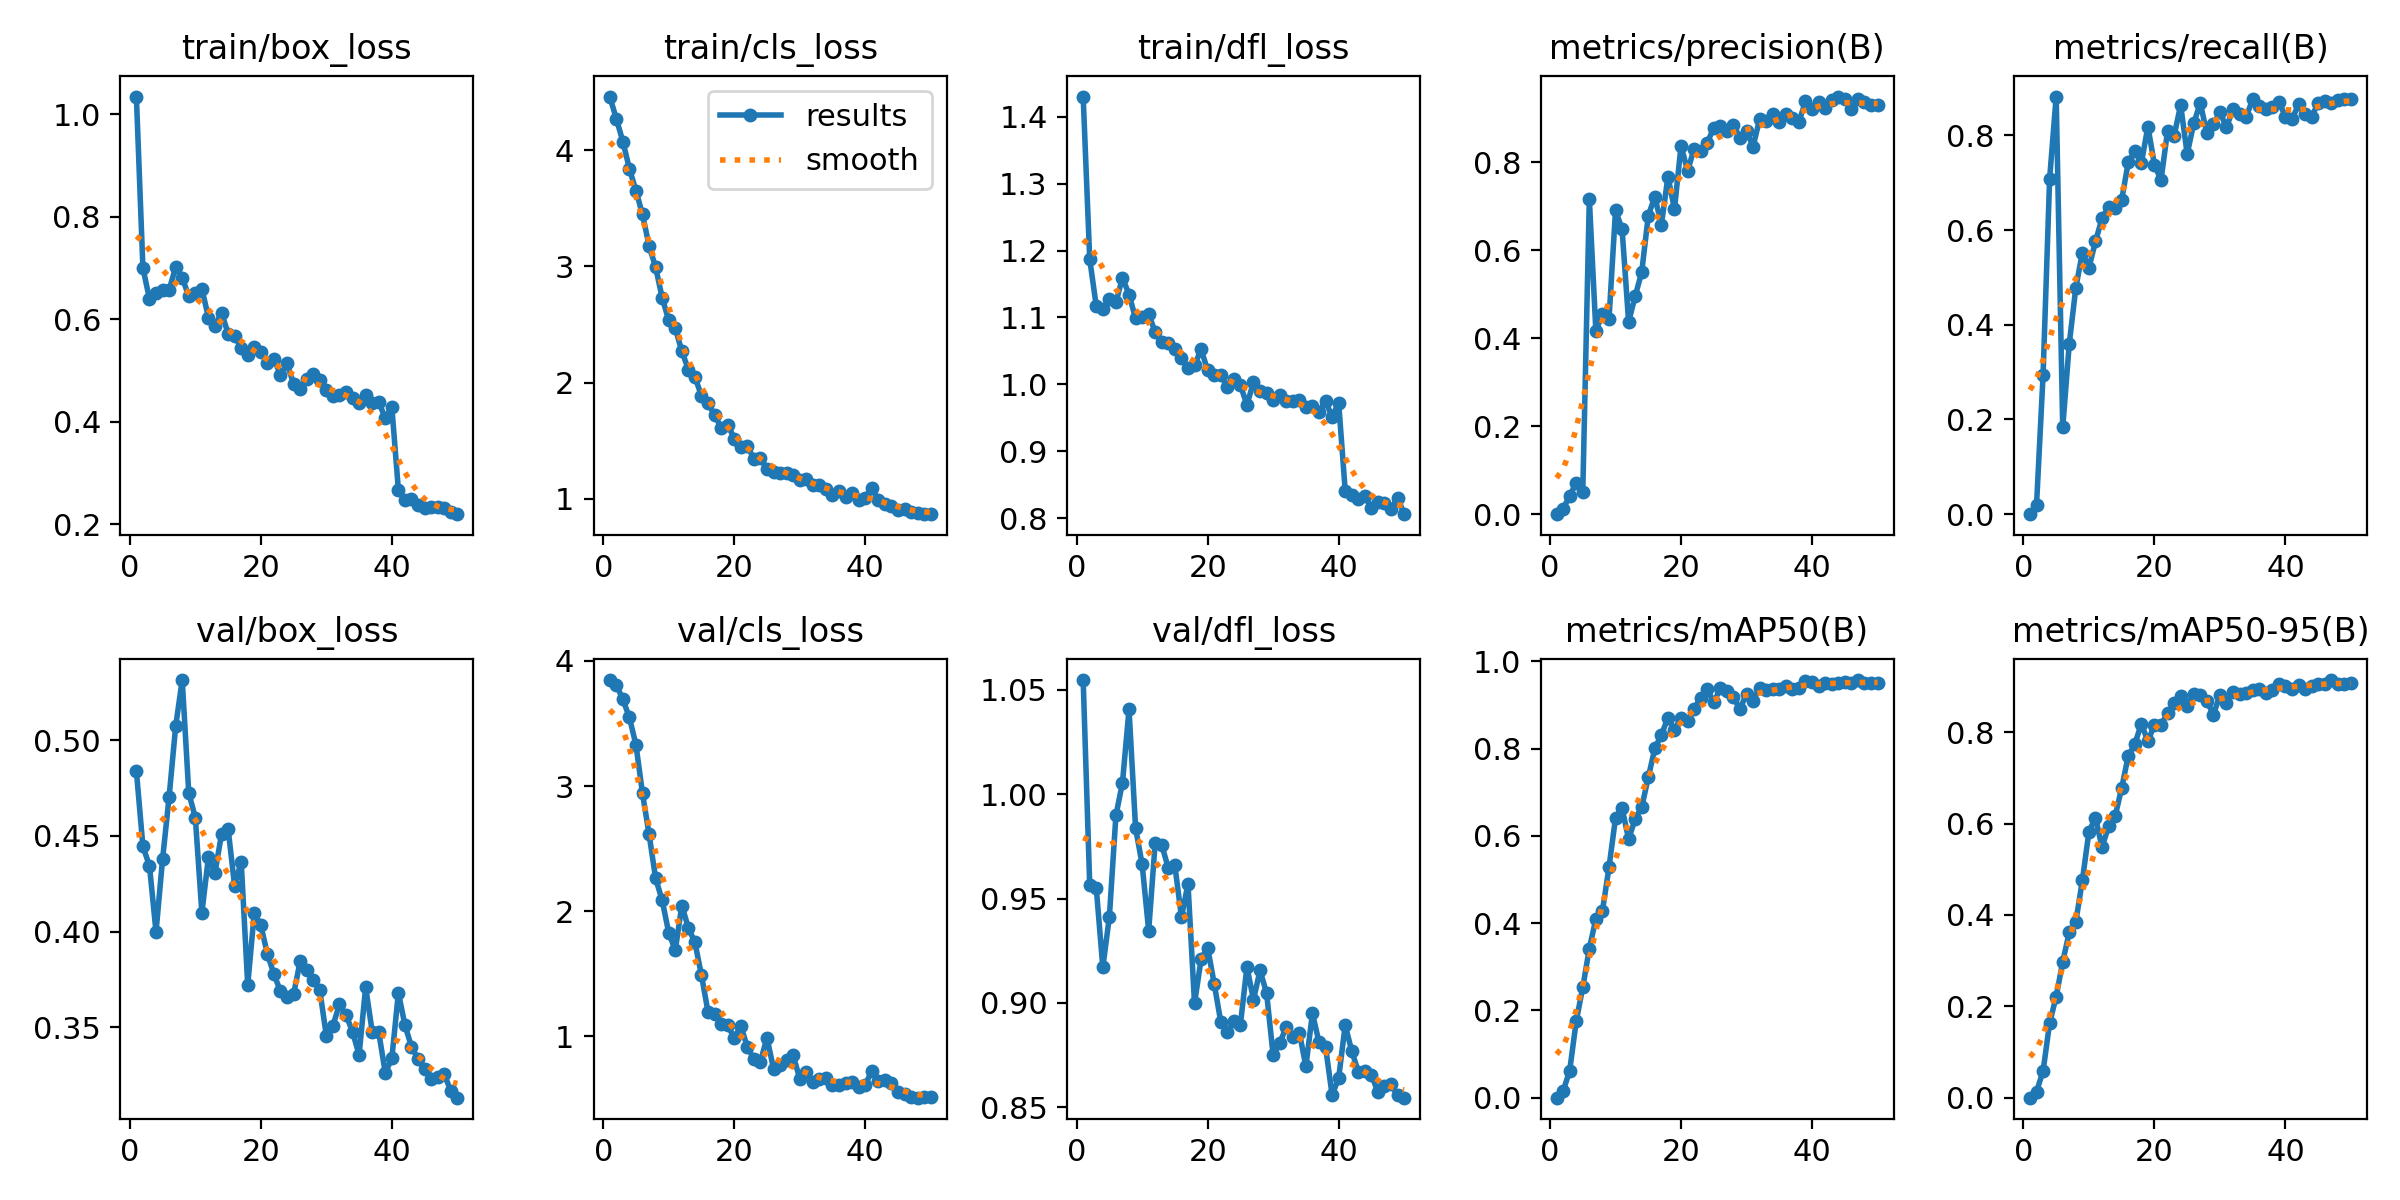
\includegraphics[width=\linewidth]{fig_yolo_training_curves.png}\\
    {\tiny YOLO11n — 50 epochs}
    \column{.48\textwidth}
    \centering
    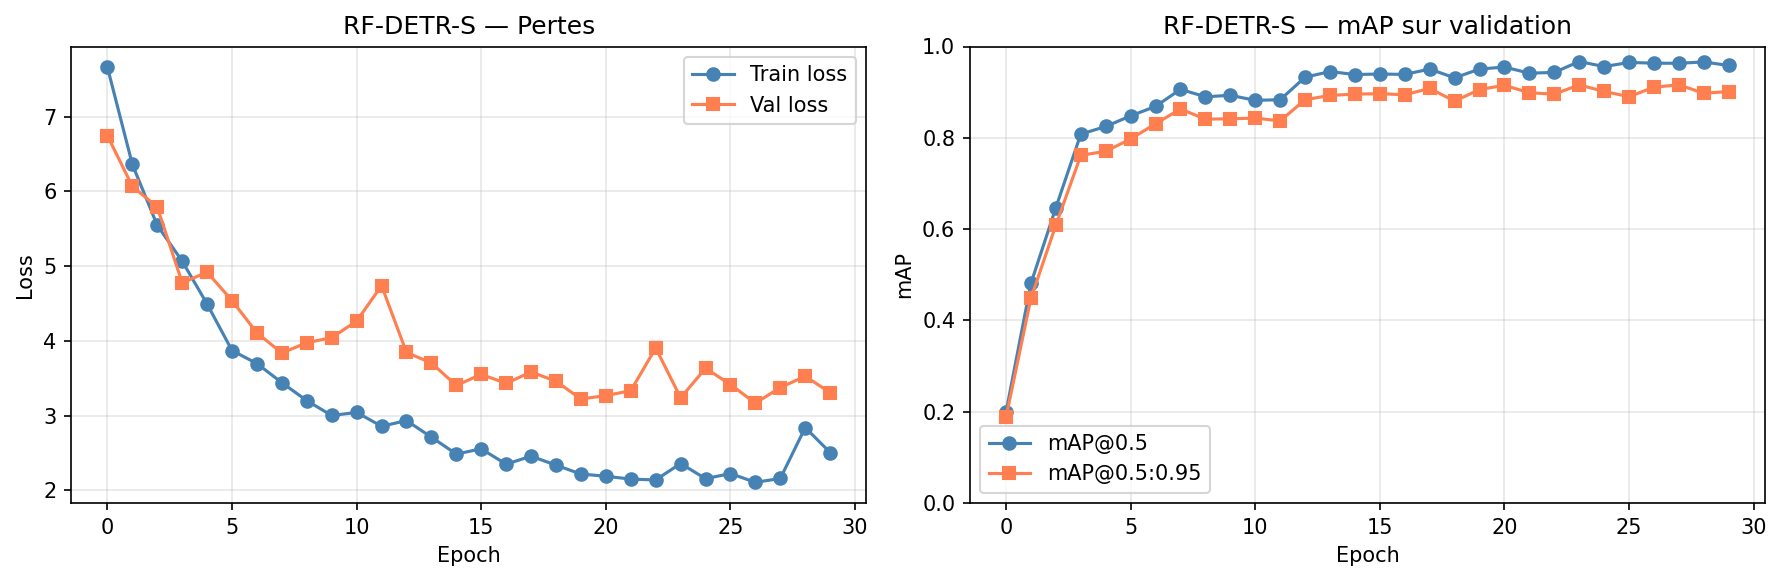
\includegraphics[width=\linewidth]{fig_rfdetr_training_curves.png}\\
    {\tiny RF-DETR-S — 30 epochs}
  \end{columns}
  \medskip
  Les deux modèles convergent rapidement grâce au pré-entraînement COCO.
\end{frame}

\begin{frame}{Performance — test set (72 images)}
  \begin{columns}[T,onlytextwidth]
    \column{.55\textwidth}
    \footnotesize
    \begin{table}
      \begin{tabular}{lcc}
        \toprule
        \textbf{Métrique} & \textbf{YOLO11n} & \textbf{RF-DETR-S} \\
        \midrule
        mAP@0.5             & \textbf{0.904} & 0.901 \\
        mAP@0.5:0.95        & 0.875 & \textbf{0.881} \\
        Précision           & 0.879 & --- \\
        Rappel              & 0.755 & --- \\
        F1-score            & 0.812 & --- \\
        \midrule
        Latence (T4)        & \textbf{36.4 ms} & 132.8 ms \\
        FPS                 & \textbf{27.5}    & 7.5      \\
        Taille              & \textbf{5.2 MB}  & 121.8 MB \\
        \bottomrule
      \end{tabular}
    \end{table}

    \column{.45\textwidth}
    \centering
    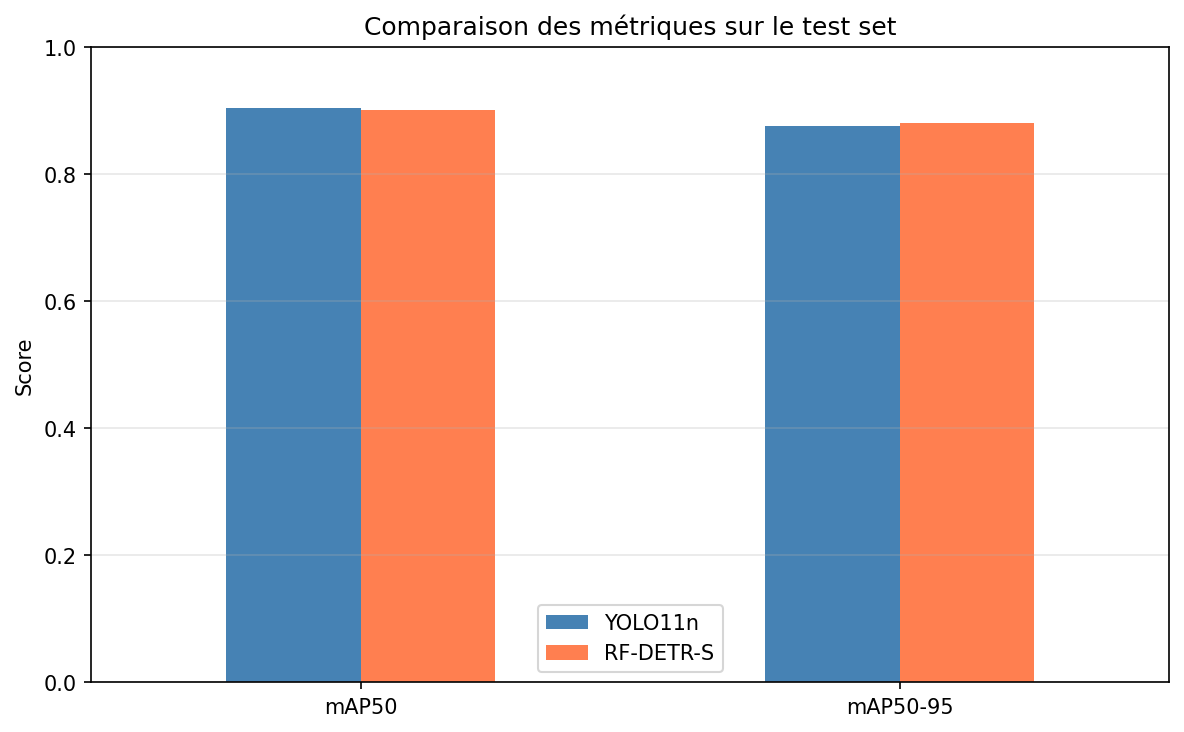
\includegraphics[width=\linewidth]{fig_comparison_metrics.png}
  \end{columns}
  \medskip
  \begin{alertblock}{Observation}
    Précision \textbf{quasi identique} ; YOLO est \textbf{$\sim$3.6$\times$ plus rapide} et \textbf{23$\times$ plus léger}.
  \end{alertblock}
\end{frame}

\begin{frame}{Étude de robustesse — point fort}
  \begin{columns}[T,onlytextwidth]
    \column{.5\textwidth}
    \centering
    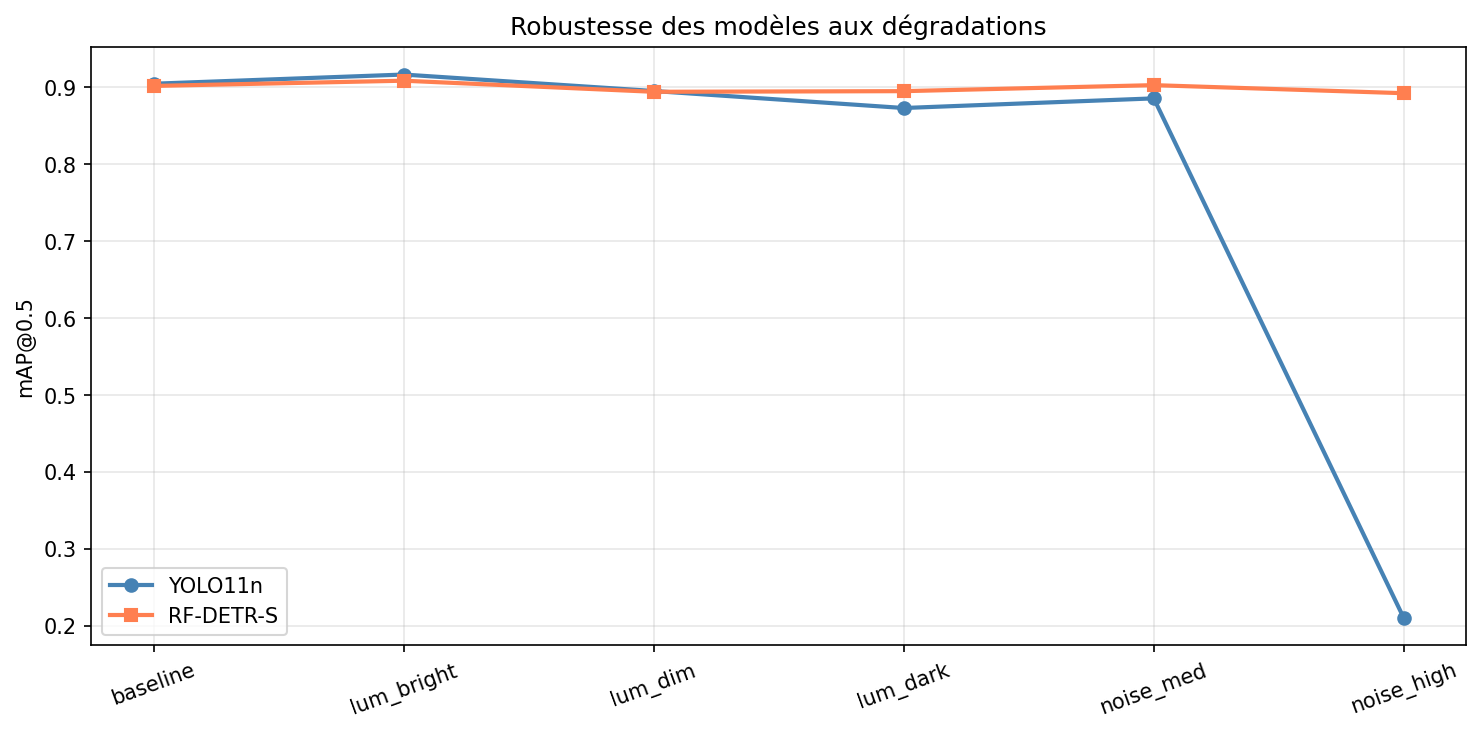
\includegraphics[width=\linewidth]{fig_robustness.png}\\
    {\tiny mAP@0.5 sous chaque condition dégradée}

    \column{.5\textwidth}
    \footnotesize
    \begin{tabular}{lcc}
      \toprule
      Cond. & YOLO $\Delta$\% & RF-DETR $\Delta$\% \\
      \midrule
      $\gamma=1.5$  & $+1.3$  & $+0.8$ \\
      $\gamma=0.75$ & $-1.0$  & $-0.8$ \\
      $\gamma=0.5$  & $-3.5$  & $-0.8$ \\
      $\sigma=15$   & $-2.1$  & $+0.1$ \\
      $\sigma=35$   & {\color{drop}\textbf{$-76.8$}} & $-1.1$ \\
      \midrule
      Moy.\,$|\Delta|$ & {\color{drop}\textbf{16.9\,\%}} & \textbf{0.7\,\%} \\
      \bottomrule
    \end{tabular}
  \end{columns}
  \medskip
  \begin{alertblock}{Découverte clé}
    \textbf{RF-DETR-S est dramatiquement plus robuste.}
    YOLO s'effondre à 0.21 mAP sous bruit fort, RF-DETR reste à 0.89.
  \end{alertblock}
\end{frame}

\begin{frame}{Pourquoi cet écart ?}
  \begin{columns}[T,onlytextwidth]
    \column{.48\textwidth}
    \begin{block}{YOLO — convolutions locales}
      \begin{itemize}
        \item Raisonne par \textbf{voisinages locaux}.
        \item Sensible aux perturbations \textbf{haute fréquence}.
        \item Effondrement quand le bruit masque les contours.
      \end{itemize}
    \end{block}

    \column{.48\textwidth}
    \begin{block}{RF-DETR — attention globale}
      \begin{itemize}
        \item Attention sur \textbf{toute l'image}.
        \item Backbone \textbf{DINOv2} pré-entraîné par auto-supervision.
        \item Représentations sémantiques \textbf{stables} face au bruit.
      \end{itemize}
    \end{block}
  \end{columns}
\end{frame}

%% ====================================================================
\section{Démonstration}

\begin{frame}{Application Gradio — 4 onglets}
  \begin{itemize}
    \item \textbf{Alphabet ASL} : grille de référence des 26 signes.
    \item \textbf{Comparaison sur image} : YOLO + RF-DETR côte à côte.
    \item \textbf{Webcam temps réel} : détection live à 27 FPS (YOLO).
    \item \textbf{Épellation} : maintenir un signe pour l'ajouter au mot.
  \end{itemize}
  \begin{block}{Déploiement public}
    \begin{itemize}
      \item Image \textbf{Docker} + reverse-proxy \textbf{Caddy} + HTTPS \textbf{Let's Encrypt}.
      \item URL : \textcolor{espblue}{\textbf{\url{https://asl-detection-yolo-rfdetr.duckdns.org/}}}
    \end{itemize}
  \end{block}
  \centering\small Webcam fonctionnelle grâce au HTTPS (contrainte navigateur).
\end{frame}

%% ====================================================================
\section{Conclusion}

\begin{frame}{Recommandation pratique}
  \begin{columns}[T,onlytextwidth]
    \column{.48\textwidth}
    \begin{block}{Choisir YOLO11n quand…}
      \begin{itemize}
        \item Conditions de capture maîtrisées.
        \item Cible \textbf{embarquée} ou \textbf{edge} (mobile, navigateur).
        \item Besoin de fluidité $>$ 25 FPS.
        \item Notre cas pour la \textbf{démo webcam}.
      \end{itemize}
    \end{block}

    \column{.48\textwidth}
    \begin{block}{Choisir RF-DETR-S quand…}
      \begin{itemize}
        \item Environnement non maîtrisé : surveillance, extérieur.
        \item Capteurs bruités, faible luminosité.
        \item GPU disponible côté serveur.
        \item Précision robuste prioritaire.
      \end{itemize}
    \end{block}
  \end{columns}
\end{frame}

\begin{frame}{Conclusion \& Perspectives}
  \begin{block}{À retenir}
    \begin{itemize}
      \item Précision \textbf{nominale comparable} (mAP@0.5 : 0.904 vs 0.901).
      \item \textbf{YOLO} = vitesse \& légèreté ; \textbf{RF-DETR} = robustesse.
      \item Le choix dépend du \textbf{contexte de déploiement}.
    \end{itemize}
  \end{block}
  \begin{block}{Perspectives}
    \begin{itemize}
      \item \textbf{Suivi} d'objets vidéo (ByteTrack) pour stabiliser la détection.
      \item Reconnaissance de \textbf{mots} via modèle séquentiel.
      \item Élargir l'étude de robustesse (occlusions, flou de mouvement).
      \item \textbf{Distillation} de RF-DETR vers une variante plus légère.
    \end{itemize}
  \end{block}
\end{frame}

\begin{frame}[standout]
  Merci pour votre attention.\\[10pt]
  \large Questions ?\\[20pt]
  \footnotesize
  \textcolor{espgold}{\textbf{Démo live}} : \texttt{asl-detection-yolo-rfdetr.duckdns.org}\\
  \textcolor{espgold}{\textbf{Code}} : \texttt{github.com/lamine-f/asl-detection-yolo-rfdetr}\\
  \textcolor{espgold}{\textbf{Modèles}} : \texttt{huggingface.co/lamine-f-edu/asl-yolo-rfdetr}
\end{frame}

\end{document}
